This section presents the definition of the objects used in the analysis: jets, electrons, muons and $\met$. 
Unless otherwise stated, the recommendations implemented in SUSYTools-00-05-00-26 tag and analysis release Base,2.0.30 
are used for all the objects.

\subsection{Jets}
\label{sec:objects_jets}

The jet selection is summarized in Table~\ref{tab:jetsdef}. Jets are reconstructed using the anti-$k_{t}$ jet algorithm~\cite{Cacciari:2008gp} with the distance parameter $R$ 
set to $0.4$ and topological clusters as input. Jets are calibrated with local cluster weighting LCW+JES scheme, which classifies topological clusters as either being of electromagnetic or hadronic origin, and based on this applies energy corrections derived from Monte Carlo simulation. 

The jets are kept only if they have $p_\mathrm{T}>20$~GeV and lie within $|\eta|<2.8$. 
In order to remove events with fake \met, an event is vetoed when a jet with quality judged as bad in {\tt VeryLoose} criterion is present.


%%%%%%%%%%%%%%%%%%%%%%%%%%%%%%%%%%%%%%%%%%%%%%%%%%%%%%%%%%%%%
\begin{table}[htb!]
\caption{Summary of the jet selection criteria. The signal jet requirements are applied on top of the preselection.}
\label{tab:jetsdef}
\begin{center}
    \begin{tabular}{|l|c|}
      \hline
      \hline
      \multicolumn{2}{|c|}{\textbf{Pre-selected jet}}\\
    \hline
      \hline
      Collection     & AntiKt4LCTopoJets \\
      \hline
      Acceptance     & $\pt > 20\,\GeV, |\eta | < 2.8$ \\
      \hline
      Overlap        & $\Delta{}R({\mathrm jet},e)$~$>$~0.2 \\
      \hline\hline
%      \multicolumn{2}{|c|}{\textbf{Signal jet}}\\
%      \hline
%     Acceptance     & $\pt > 40\,\GeV,$ \\
%      & $|\eta | < 2.8$ \\ 
%     \hline
%      \hline
      \multicolumn{2}{|c|}{\textbf{b-jets}}\\
    \hline
      \hline
     Acceptance     & $\pt > 20\,\GeV,$ \\
      & $|\eta | < 2.5$ \\ 
      \hline
     b-tagging  &  MV1 algorithm 70\% OP\\
      \hline
\end{tabular}
\end{center}
\end{table}
%%%%%%%%%%%%%%%%%%%%%%%%%%%%%%%%%%%%%%%%%%%%%%%%%%%%%%%%%%%%

\subsubsection{Jet Vertex Fraction}
During Run-1, in many analyses a Jet Vertex Fraction ({\sc JVF}) cut was applied  to jets with $\pT < 50 \GeV$ and $| \eta | < 2.4$ to mitigate the effects of pileup. JVF is reported to be buggy in DC14 samples due to lacking a proper track selection for the computation of this variable. Figure~\ref{fig:jvf_deltaR} shows the distribution of JVF as a function of the $\Delta R$ between the jet and the nearest truth jet originated from the hard scattering for jets with $\pT < 50 \GeV$ and $| \eta | < 2.4$ in a DC14 $\ttbar +W$ sample. 
Despite the technical problem mention above, most of the reconstructed jets not originated from the hard scattering have JVF$<$0.5. 
Nevertheless, the distribution for jets well matched to truth jets is very flat, and applying a cut on JVF would lead to 
low efficiency on jets originated from the hard scattering.


\begin{figure}[htb!!]
\begin{center}
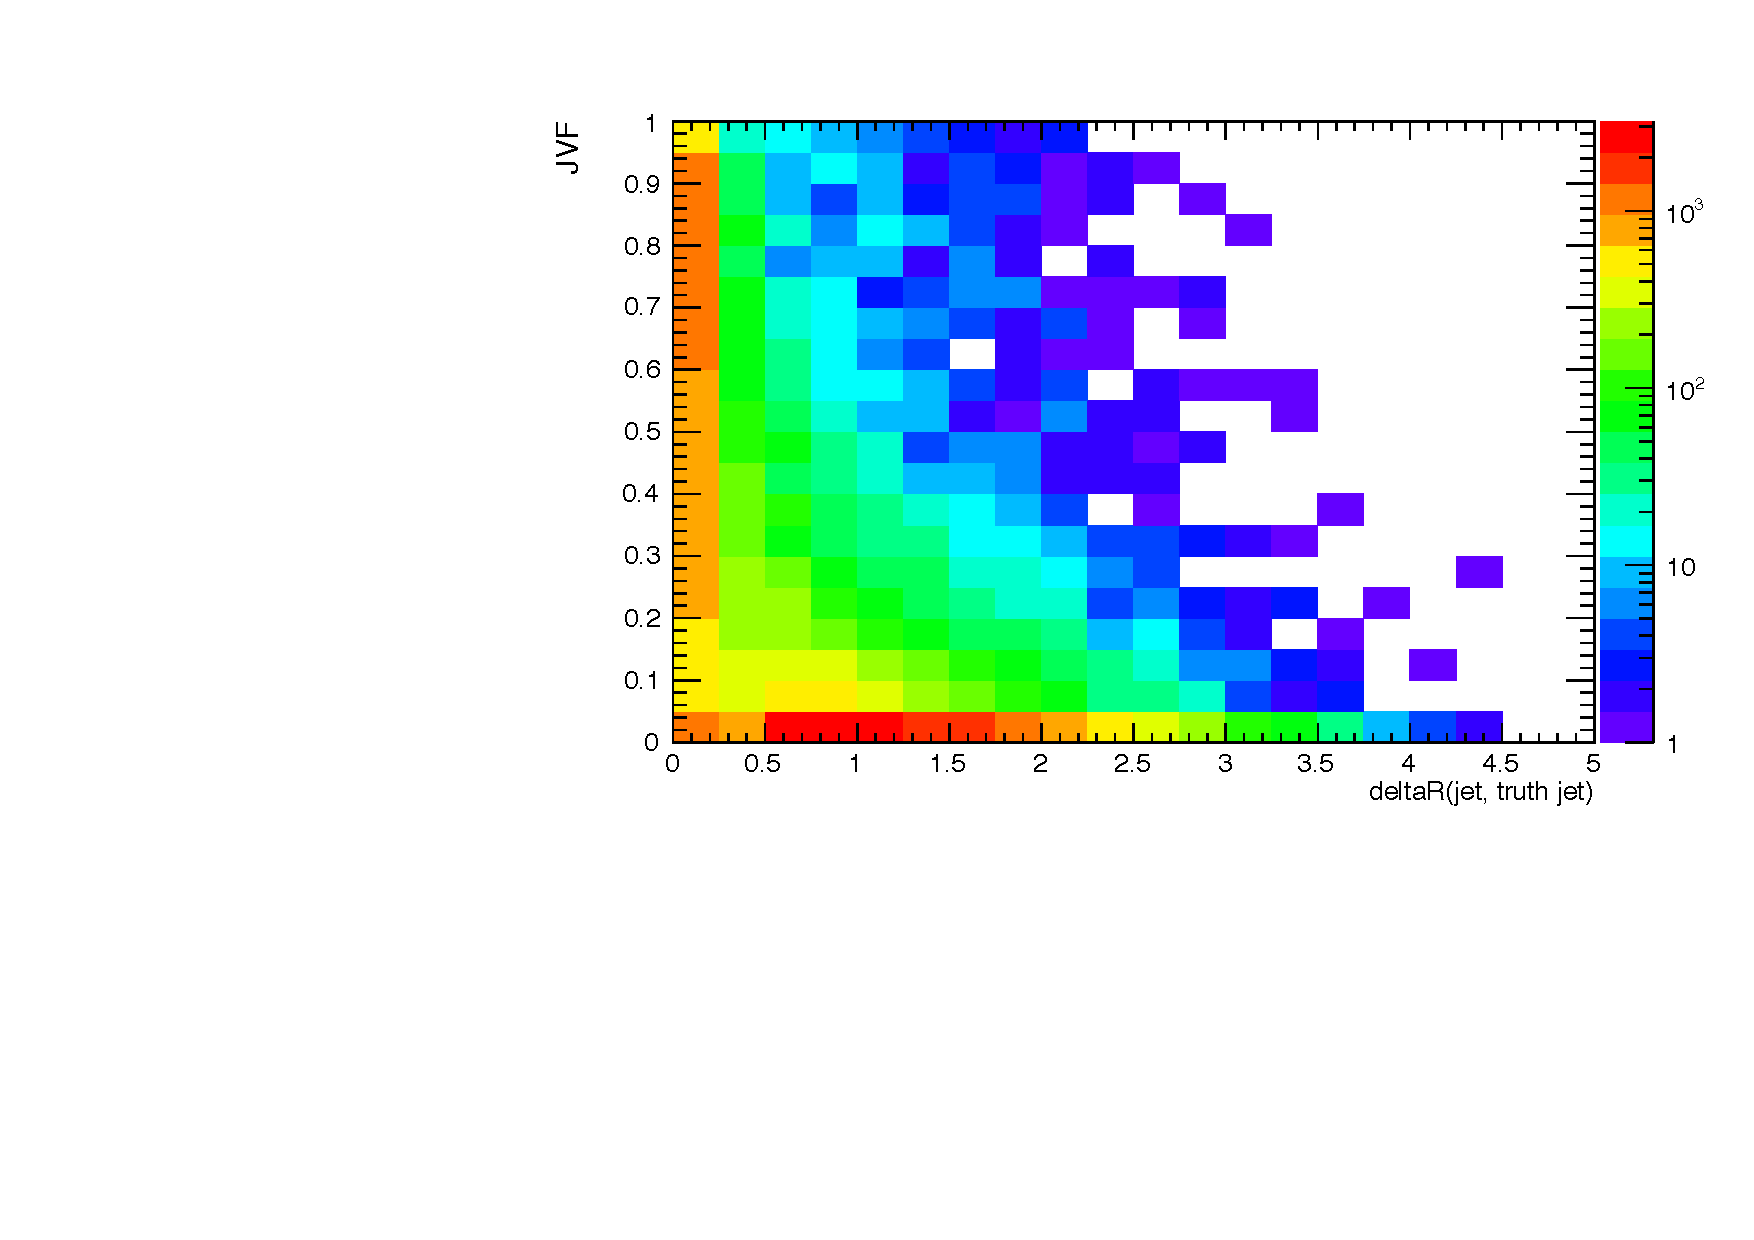
\includegraphics[scale=0.38]{jvf_deltaR.pdf}
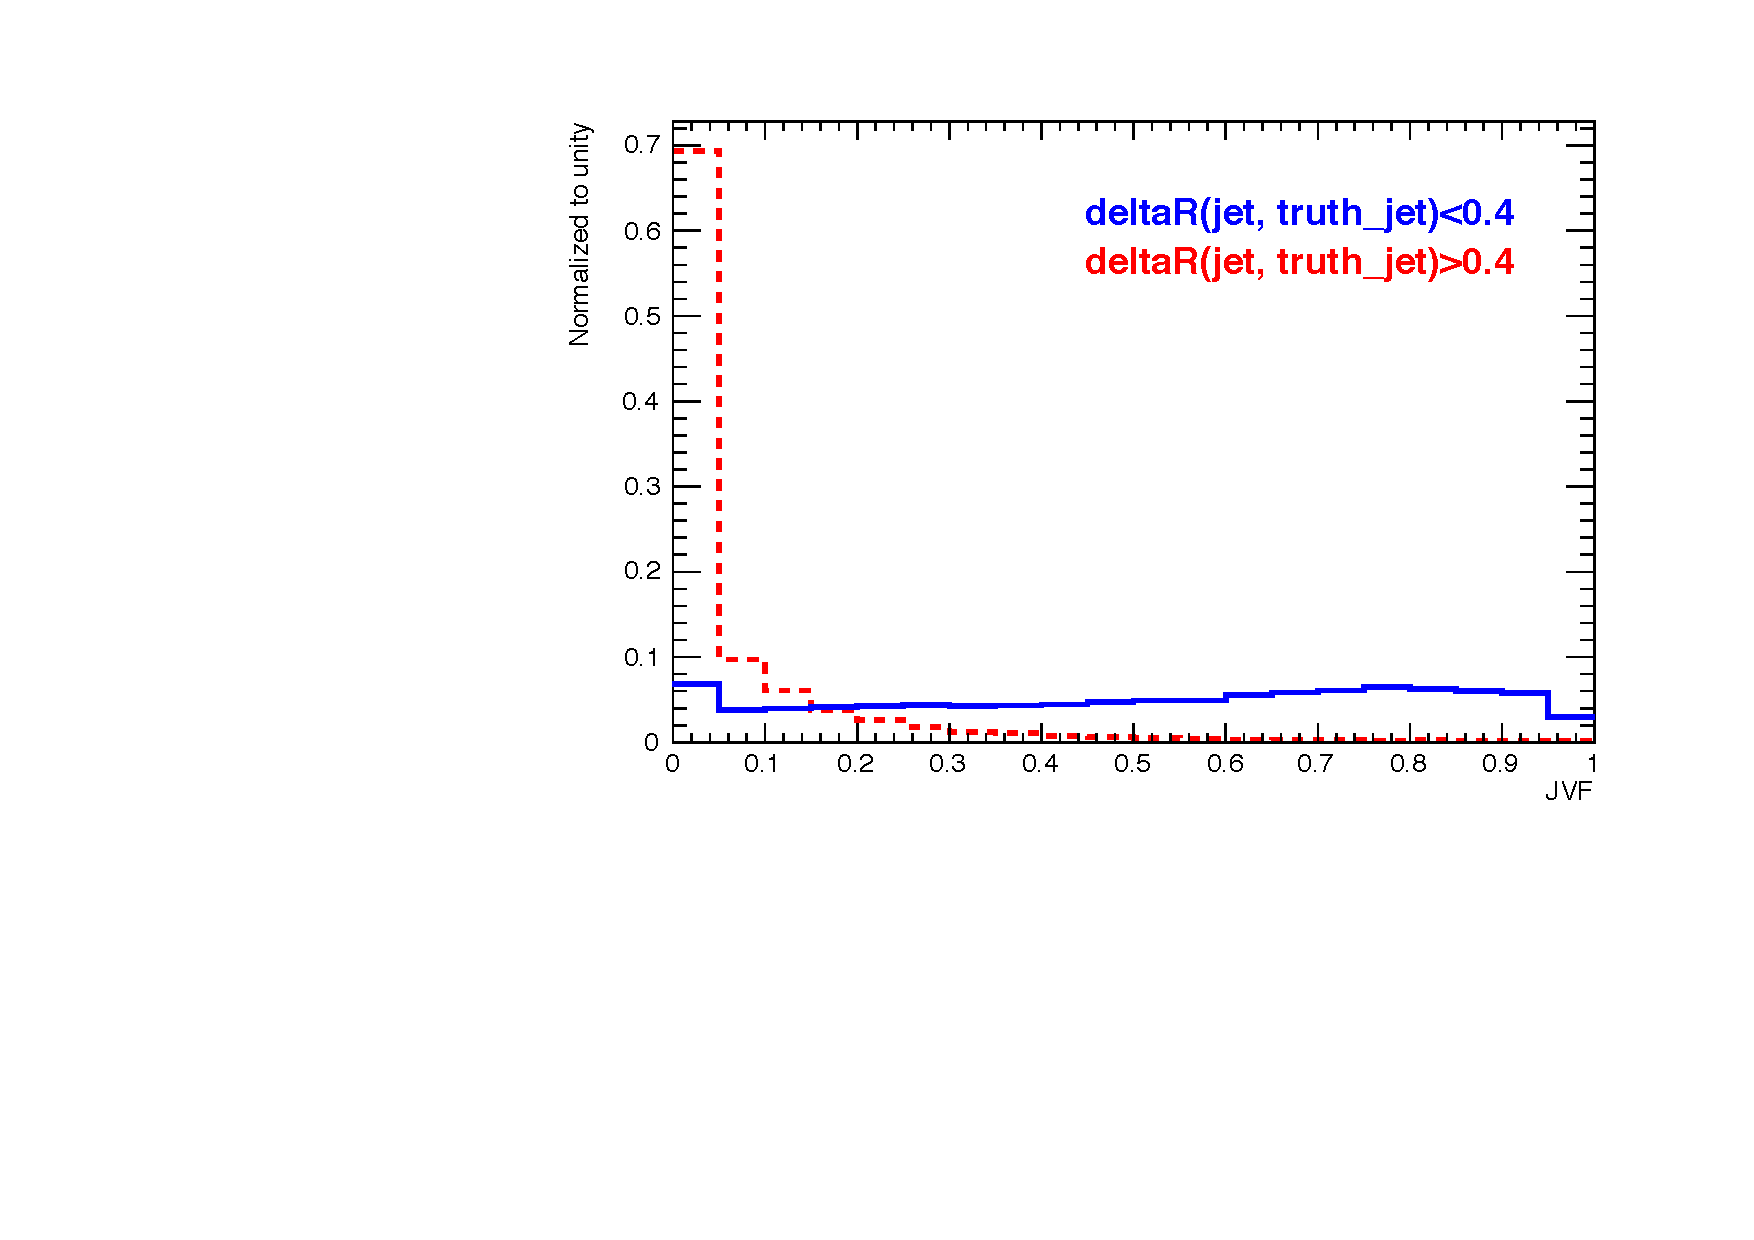
\includegraphics[scale=0.38]{jvf_1d_deltaR.pdf}
\end{center}
\vspace{-0.2cm}
\caption{On the left, jet vertex fraction as a function of the distance between the reconstructed jet and the nearest truth jet originated from the hard scattering in a $\ttbar+W$ sample. On the right, jet vertex fraction distribution for jets with $\Delta R$ values below and above 0.4. Only jets with $\pT < 50 \GeV$ and $| \eta | < 2.4$ are included in the plots.}
\label{fig:jvf_deltaR}
\end{figure}

\subsubsection{$b$-tagging}

Tagging of jets is done using the MV1 algorithm as included in DC14 with the 70\% efficiency 
operating point. This algorithm is based on a neural network using 
the output weights of the JetFitter+IP3D, IP3D and SV1 algorithms as input.

Note that MV1 will be superseded by MV2c in MC15 productions (release 20), with better background rejection and signal efficiency. 
The Flavor Tagging CP group also recently released 20-like ($\pT$, $\eta$) efficiency and mis-tag maps obtained from $\ttbar$ to be used in DC14 samples, which could not be used for this note due to lack of time.


%The $b$ jets used in the hadronic $m_\textup{T2}$ analysis are tagged using the MV1 tagging algorithm, at the 70\% working point. The event weights applied to MC to correct for differences in $b$ tagging efficiency between data %and MC are the so-called ``$t\bar{t}$ event weights'' (latest 2013 recommendations, named ``KinSel\_dilep'' in %the .root file which provides the calibrations) computed on jets to which a JVF cut has been applied. The bulk of the %$b$ jets entering the SR and CR for this analysis lie in the region $50<p_\mathrm{T}<200$~GeV. In this region the %agreement between the $b$ jet $p_\mathrm{T}$ distributions in data and MC in events with 2 $b$ jets is best when %the $t\bar{t}$ weights are chosen. This choice has also been found to be best for other SUSY analyses using a 2 $b%$ jet selection.


\subsection{Leptons}
\label{sec:objects_leptons}

This section summarizes the electron and muon object selection, as well as developments done in the optimization of the
lepton isolation and electron acceptance cuts.

\subsubsection{Electrons}
\label{sec:objects_electrons}

The electron selection is summarized in Table~\ref{tab:lepdef}. The Egamma CP group recommends the likelihood-based electron identification~\cite{ATLAS-CONF-2014-032} for Run-2, since it provides a factor of two better background rejection than the cut-based identification.
Four working points ({\tt VeryLooseLLH}, {\tt LooseLLH}, {\tt MediumLLH}, {\tt TightLLH}) are available for LLH electrons.

Pre-selected electrons must satisfy the {\tt LooseLLH} requirements defined by the Egamma group and have $E_\mathrm{T}>10$~GeV and $|\eta|<2.47$. Signal electrons are additionally required to pass the isolation cuts defined in~\ref{sec:isolation} as well as 
the {\tt TightLLH} identification criteria.

A multiplicative event weight is applied for each selected electron to the overall event weight in order to correct for differences in efficiency between data and MC as recommended by the Egamma group.

\subsubsection{Muons}
\label{sec:objects_muons}

The muon selection is summarized in Table~\ref{tab:lepdef}. The Run-2 muon PID is provided by the so-called \textit{third chain}: 
this has been designed to provide the best performances from Run-1 STACO and MUID chains. The following working points are supported:
{\tt Tight}, {\tt Medium}, {\tt Loose} and {\tt VeryLoose}. 

Pre-selected muon candidates must pass the {\tt Medium} muon quality cuts and have  $p_\mathrm{T} > 10\GeV$ and $|\eta| < 2.4$.
A smearing procedure is applied to the muon $p_\mathrm{T}$.  A multiplicative event weight is applied for each selected muon to the overall event weight in order to correct for differences in efficiency between data and MC as recommended by the Muon CP group. 

Finally, signal muon candidates have been required to pass the isolation cuts defined in~\ref{sec:isolation}.

Note that events with ``cosmic'' muons, or ``Bad'' muon are vetoed as described in Section~\ref{sec:presel}.


%%%%%%%%%%%%%%%%%%%%%%%%%%%%%%%%%%%%%%%%%%%%%%%%%%%%%%%%%%%%%
\begin{table}[htb!]
\caption{Summary of the electron and muon selection criteria. The signal
  selection requirements are applied on top of the preselection. The
  lepton-jet isolation requirement is applied after electron-jet overlap
  removal.}
\label{tab:lepdef}
\begin{center}
    \begin{tabular}{|l|c|c|}
      \hline
      \hline
       & \textbf{Pre-selected Electron} & \textbf{Pre-selected Muon} \\
      \hline
      \hline
      Acceptance     & $\pt > 10\,\GeV, |\eta^\mathrm{clust}| < 2.47$  & $\pt > 10\,\GeV, |\eta| < 2.4$ \\
      \hline
      Quality & {\tt LooseLLH} & {\tt{xAOD::Muon::Medium}} \\
      \hline
      Impact parameter &  $|d_0/\sigma(d_0)|<$ 5.0 & - \\
      \hline
      $\ell$-jet Isolation      & $\Delta{}R(e,jet)$~$>$~0.4 & $\Delta{}R(\mu,jet)$~$>$~0.4 \\
      \hline\hline
       & \textbf{Signal Electron} & \textbf{Signal Muon} \\
      \hline
      \hline
      Quality & {\tt TightLLH} & -\\
      \hline
      Track Isolation       & ptvarcone20/\pt$<$0.06  & ptvarcone30/\pt\ $<0.06$\\
      Calorimeter Isolation & topoetcone20/\pt$<$0.06  & - \\
      \hline
      Impact parameter & $|z_0 \cdot sin(\theta)|<$ 0.4 mm   & $|z_0 \cdot sin(\theta)|<$ 0.4 mm \\ 
      & $|d_0/\sigma(d_0)|<3.0$  & $|d_0/\sigma(d_0)| < 3.0$\\
     \hline
\end{tabular}
\end{center}
\end{table}
%%%%%%%%%%%%%%%%%%%%%%%%%%%%%%%%%%%%%%%%%%%%%%%%%%%%%%%%%%%%


\subsubsection{Lepton isolation}
\label{sec:isolation}

The lepton isolation variables contained a number of bugs/issues in the DC14 xAOD productions, which made them unusable for analysis. 
In particular, track isolation variables lacked a proper track selection (eg: $z_0$ selection), and 
calorimeter isolation variables had missing or wrong $\pt$ and pileup corrections. A fix for those problems was provided 
in the derivation framework cache 19.1.4.5, which made the isolation variables essentially identical to those being 
developed for release 20.

The isolation variables are provided for three different cone sizes: 0.2 ({\tt cone20}), 0.3 ({\tt cone30}) 
and 0.4 ({\tt cone40}), and are the following:
\begin{itemize}
\item \textbf{ptcone}: sum of the $\pt$ of tracks in the given cone around the object of interest
\item \textbf{topoetcone}: sum of transverse energy of the topological energy clusters in the calorimeter in the given cone 
around the object of interest. Unlike in Run-1, this variable is now available for both electrons and muons. 
\item \textbf{ptvarcone} (known as mini-isolation during Run-1):  sum of the $\pt$ of tracks in a cone around the object 
with radius being the smallest between the given cone size or 10~GeV/$\pt$[GeV] (where $\pt$ is the $\pt$ of the lepton). 
This definition effectively uses narrower cones for high-$\pt$ leptons, 
for instance ptvarcone30 deviates from ptcone30 only above 33.3~GeV.
\end{itemize}

Dedicated optimizations were performed about the lepton isolation, exploring track and calorimeter isolation variables 
with different cone sizes and cut values. Since this analysis is dominated by the non-prompt lepton background,  
an excellent rejection against this background is needed to keep a good signal sensitivity. This should be balanced with 
the fact the signal acceptance to SS/3L is typically low due to the leptonic branching ratio of $W$/$Z$ bosons, and it is therefore 
also essential to keep the signal efficiency as high as possible.

\paragraph{Optimization procedure}

For optimization of the isolation variables, the per-lepton efficiency is computed as the ratio of number of leptons passing a given
isolation criteria over the total number of leptons. For this ratio, the denominator is defined as all the leptons passing the 
pre-selection in SS/3L events defined in Table~\ref{tab:lepdef}, after applying the same signal lepton impact parameter cuts as in Run-1. 
The numerator is defined 
as the number of leptons additionally passing the isolation cuts as well as the electron {\tt MediumLLH}/{\tt TightLLH} identification criteria.
The isolation efficiency for non-prompt leptons in a $\ttbar$ sample is plotted as function of the efficiency for prompt 
leptons in signal events for different relative isolation cut values raging from 0 to 0.20 in steps of 0.01.

In addition, a single point corresponding to the Run-1 settings is also shown for comparison. Table~\ref{tab:run1def} shows 
the details of the isolation criteria used in Run-1. Since some of those variables are not supported anymore, 
in this study tight++ is replaced by {\tt MediumLLH} for electrons, and etcone by topoetcone in the case of muons.

%%%%%%%%%%%%%%%%%%%%%%%%%%%%%%%%%%%%%%%%%%%%%%%%%%%%%%%%%%%%%
\begin{table}[htb]
\caption{Summary of the signal electron and signal muon selection criteria used in Run-1. }
\label{tab:run1def}
\begin{center}
    \begin{tabular}{|l|c|c|} \hline
       & Run-1 Signal Electron & Run-1 Signal Muon \\
      \hline
      \hline
      Quality & {\tt Tight++} & -\\
      \hline
      Track Isolation       & ptcone20/min(\pt, $60\gev$)\ $<0.06$  & ptcone30/min(\pt, $60\gev$)\ $<0.12$\\
      Calorimeter Isolation & topoEtcone20/min(\pt, $60\gev$)\ $<0.06$ & etcone30/min(\pt, $60\gev$)\ $<0.12$\\
      \hline
      Impact parameter & $|z_0 \cdot sin(\theta)|<$ 0.4 mm   & $|z_0 \cdot sin(\theta)|<$ 0.4 mm \\ 
      & $|d_0/\sigma(d_0)|<3.0$  & $|d_0/\sigma(d_0)| < 3.0$\\
     \hline
\end{tabular}
\end{center}
\end{table}
%%%%%%%%%%%%%%%%%%%%%%%%%%%%%%%%%%%%%%%%%%%%%%%%%%%%%%%%%%%%

\paragraph{Variable selection for muons}

Figure~\ref{fig:isoMuon} shows the isolation efficiency for muons using several variables. As shown, if relying on cone20 variables, 
both track and calorimeter isolation would be needed to bring the background rejection to levels comparable to those used in Run-1, particularly at muon $\pt$ below 40~GeV. On the contrary, using cone30 variables a similar performance as during Run-1 can be 
achieved even at low $\pt$. In addition, using track isolation can provide larger signal efficiency than a combined track+calo 
isolation for any given background rejection. Comparing the two possible choices for track isolation, ptvarcone provide about 5\% 
extra signal efficiency for signal at $\pt>40$~GeV. Therefore, ptvarcone30 is chosen as the only variable to be used for muon 
isolation due to its good signal efficiency at high $\pt$ together with a very good background rejection at low $\pt$.

\begin{figure}[phtb!]
\begin{center}
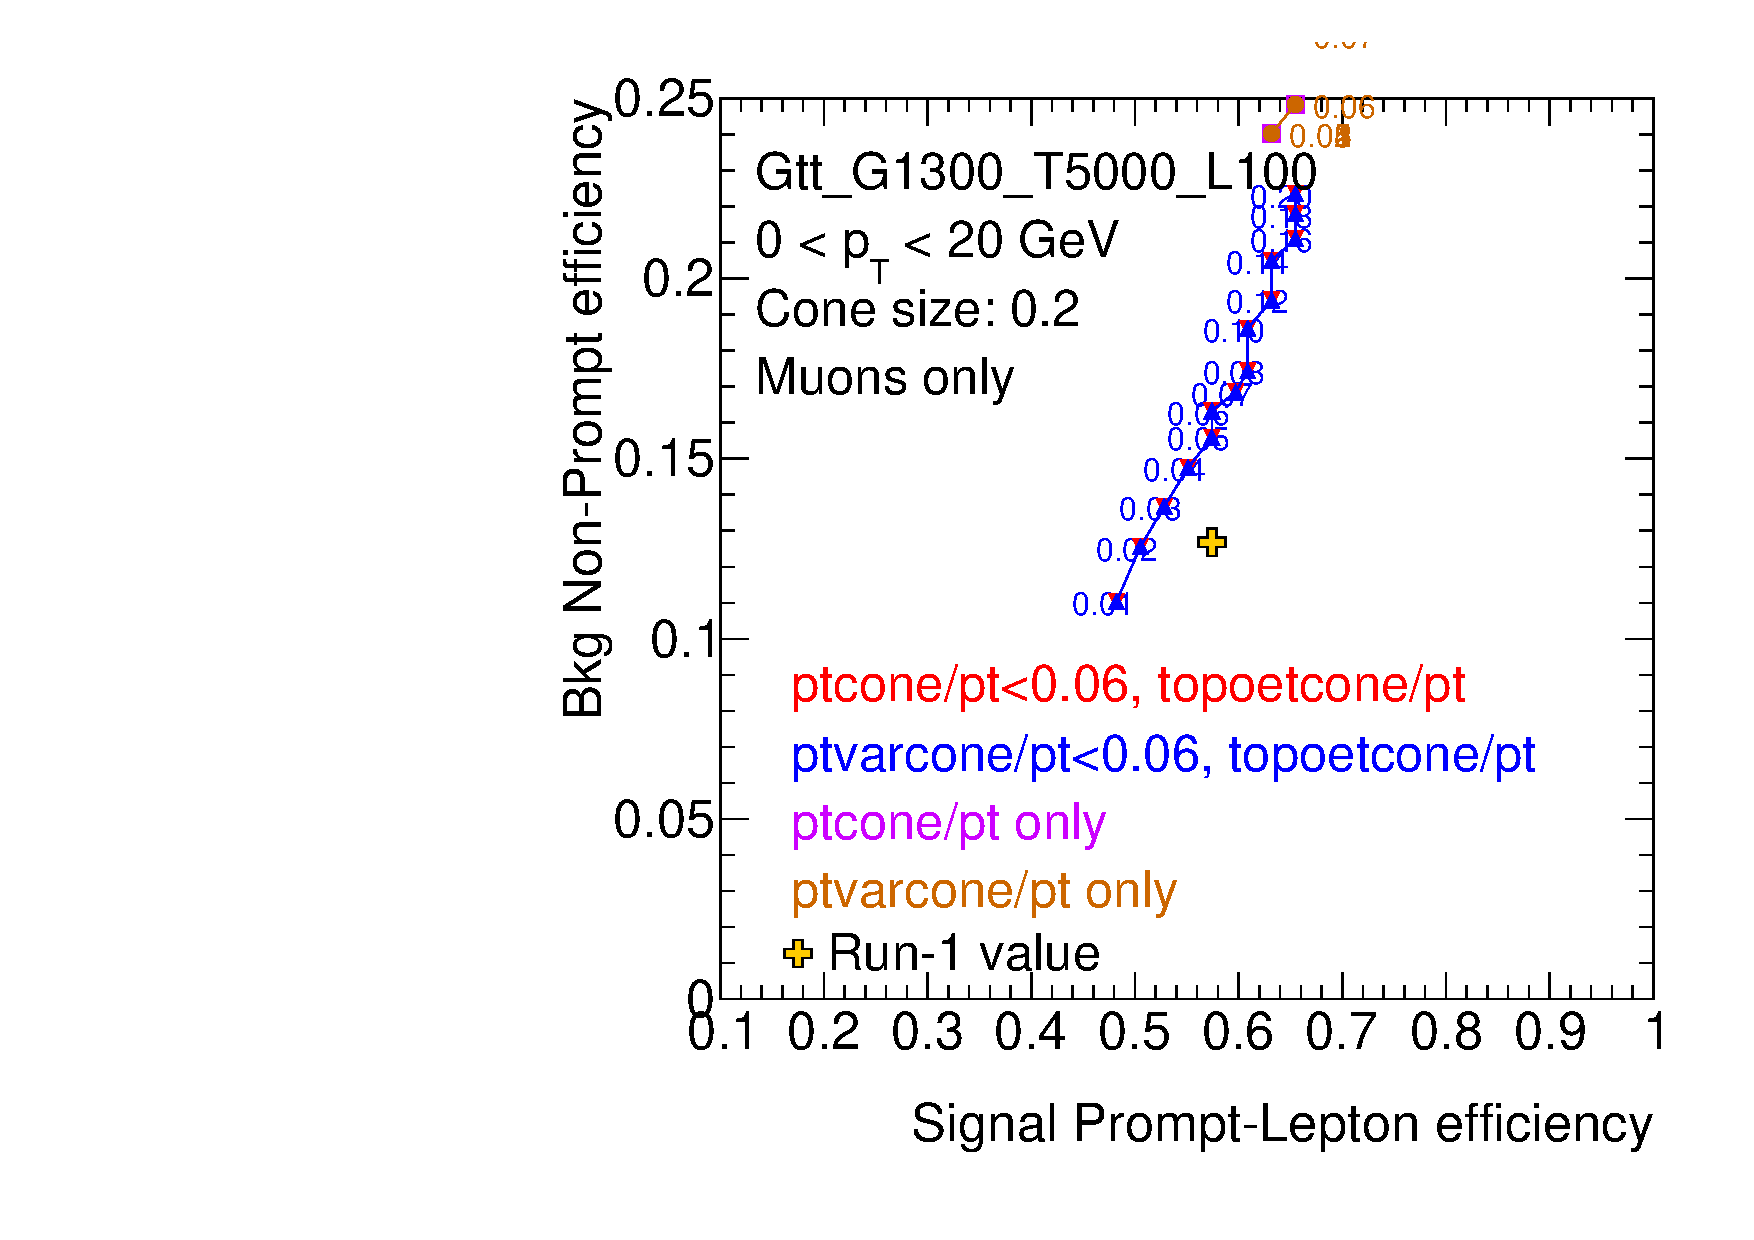
\includegraphics[page=1,width=0.4\textwidth]{FIGURES/ISOLATION/isoMu.pdf}
\includegraphics[page=7,width=0.4\textwidth]{FIGURES/ISOLATION/isoMu.pdf}
\includegraphics[page=2,width=0.4\textwidth]{FIGURES/ISOLATION/isoMu.pdf}
\includegraphics[page=8,width=0.4\textwidth]{FIGURES/ISOLATION/isoMu.pdf}
\includegraphics[page=3,width=0.4\textwidth]{FIGURES/ISOLATION/isoMu.pdf}
\includegraphics[page=9,width=0.4\textwidth]{FIGURES/ISOLATION/isoMu.pdf}
%\includegraphics[page=4,width=0.4\textwidth]{FIGURES/ISOLATION/isoMu.pdf}
%\includegraphics[page=10,width=0.4\textwidth]{FIGURES/ISOLATION/isoMu.pdf}
\end{center}
\vspace{-0.2cm}
\caption{Isolation efficiency for background non-prompt muons as a function of the isolation efficiency for prompt muons in signal events for cone20 variables (left) and cone30 variables (right) in different muon $\pt$ bins. Curves are shown for ptcone alone, ptvarcone alone, ptcone combined with topoetcone as well as for ptvarcone combined with topoetcone. In addition, the cross shows the value that would be obtained with settings equivalent to those used during Run-1.}
\label{fig:isoMuon}
\end{figure}

\paragraph{Variable selection for electrons}

Figure~\ref{fig:isoEl1} compares the performances of several isolation cones in the case of electrons. As shown, only combining calorimeter and track isolation and using cone20 variables similar efficiency/rejection performance to that in Run-1 can be achieved.  
  
\begin{figure}[phtb!]
\begin{center}
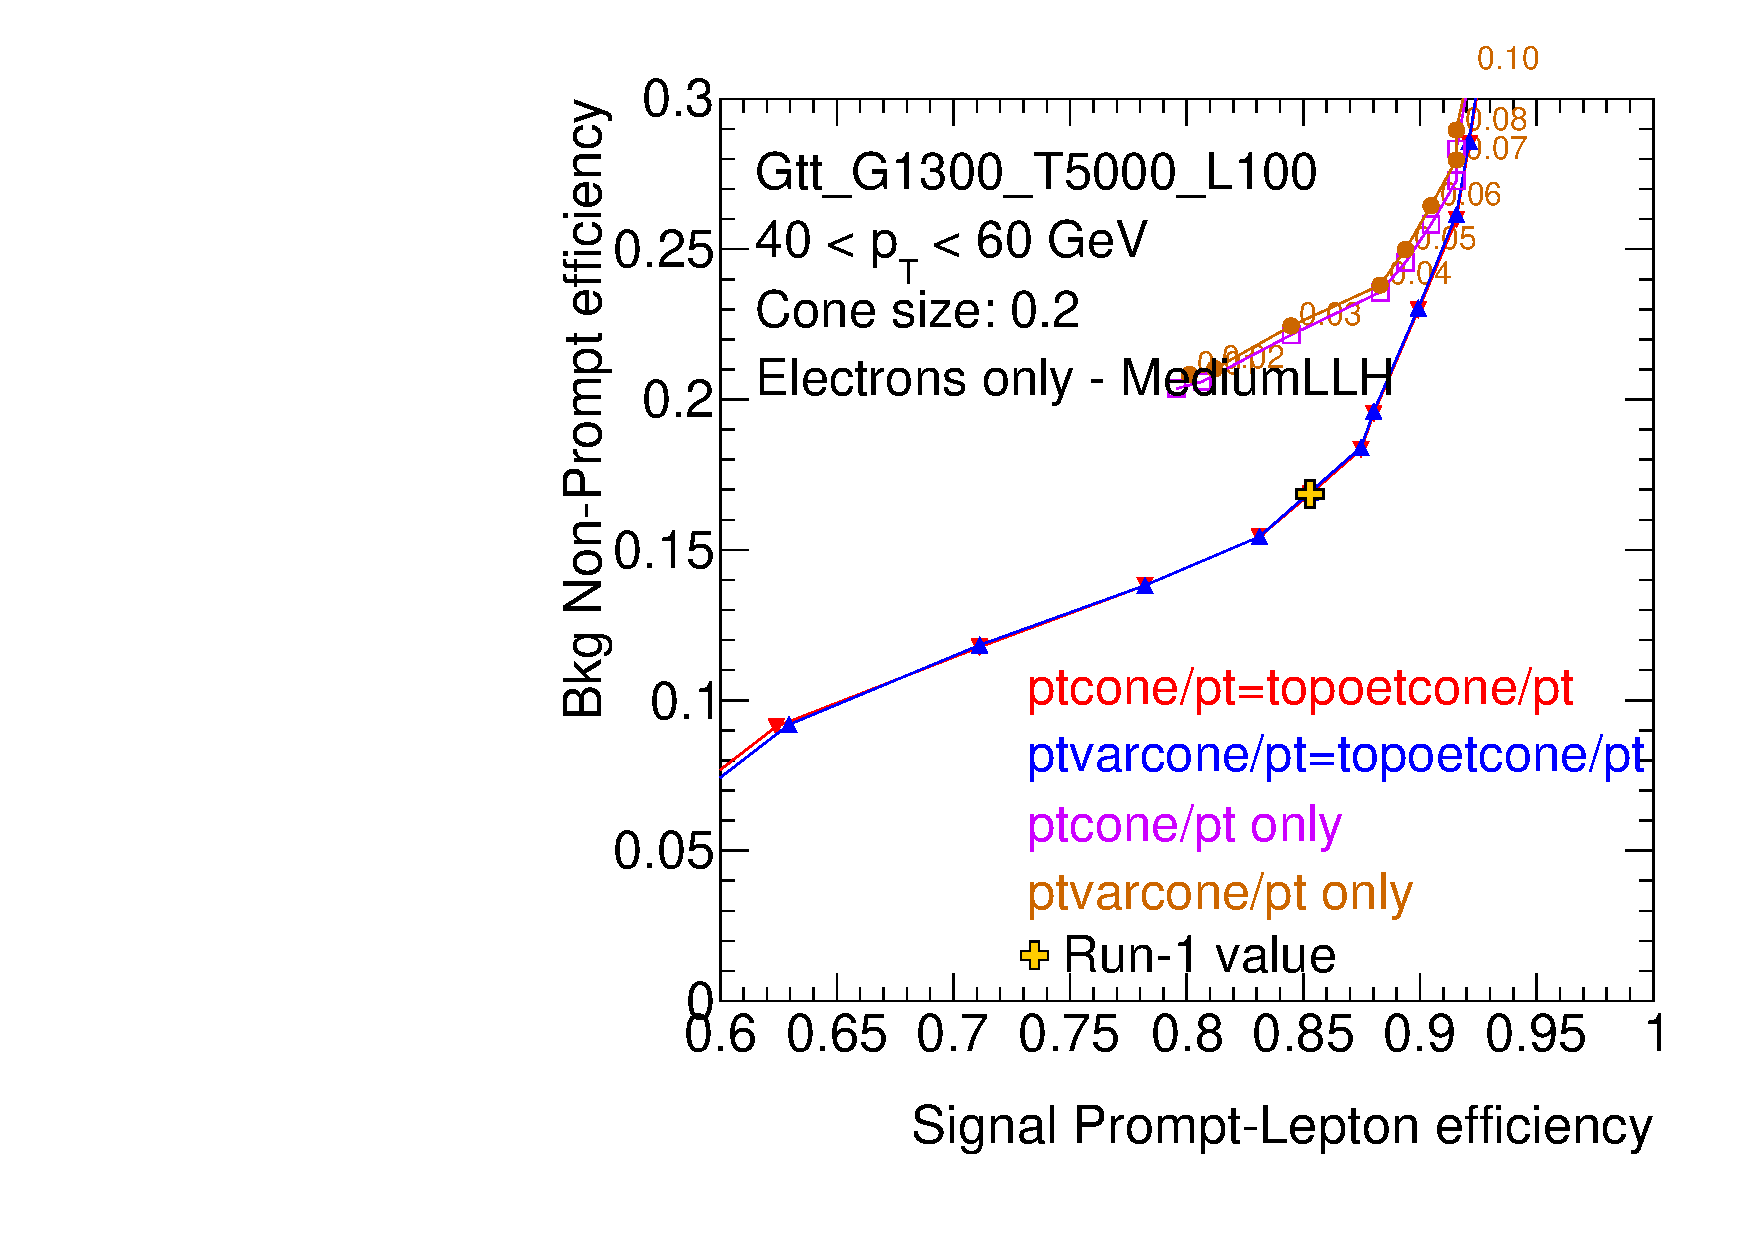
\includegraphics[width=0.4\textwidth]{FIGURES/ISOLATION/Gtt_G1300_T5000_L100_pt3-3_cone20_id11_med.pdf}
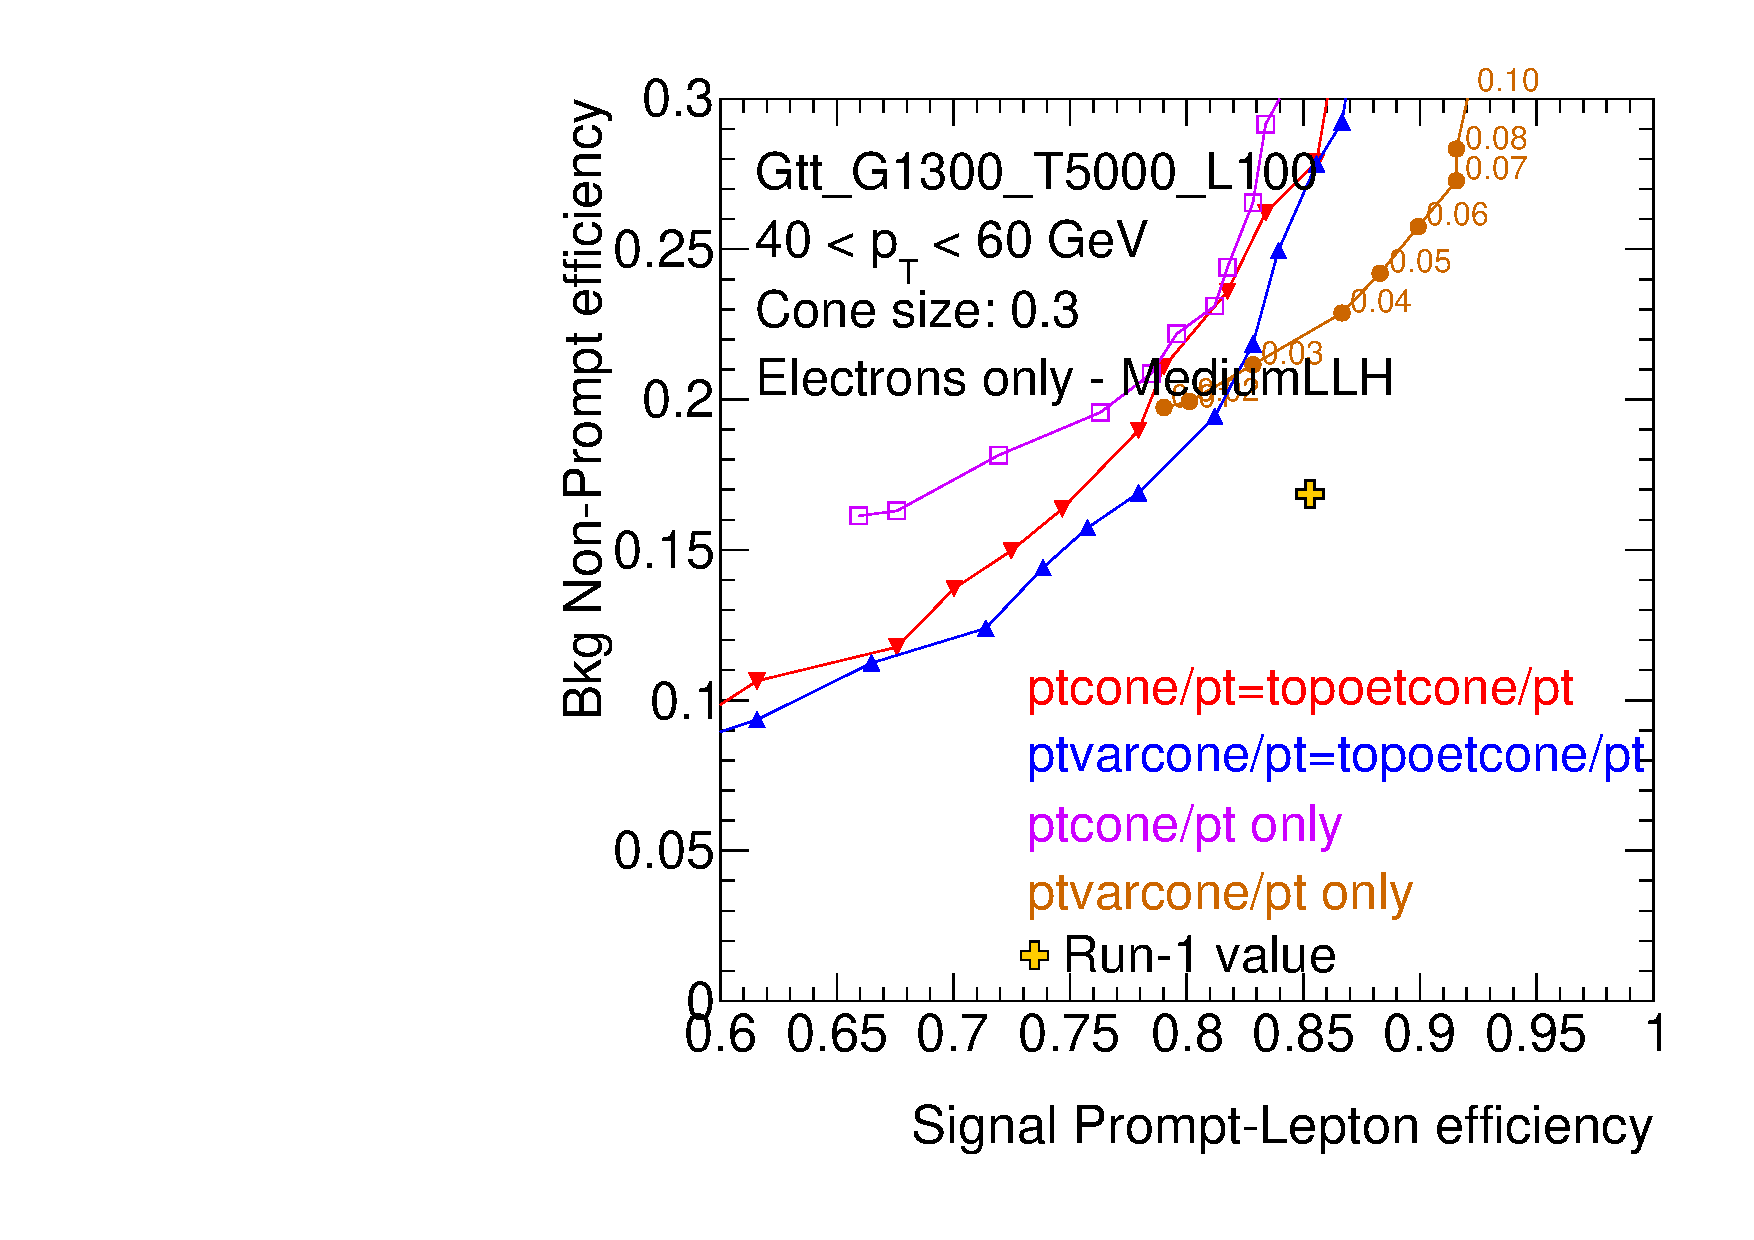
\includegraphics[width=0.4\textwidth]{FIGURES/ISOLATION/Gtt_G1300_T5000_L100_pt3-3_cone30_id11_med.pdf}\\
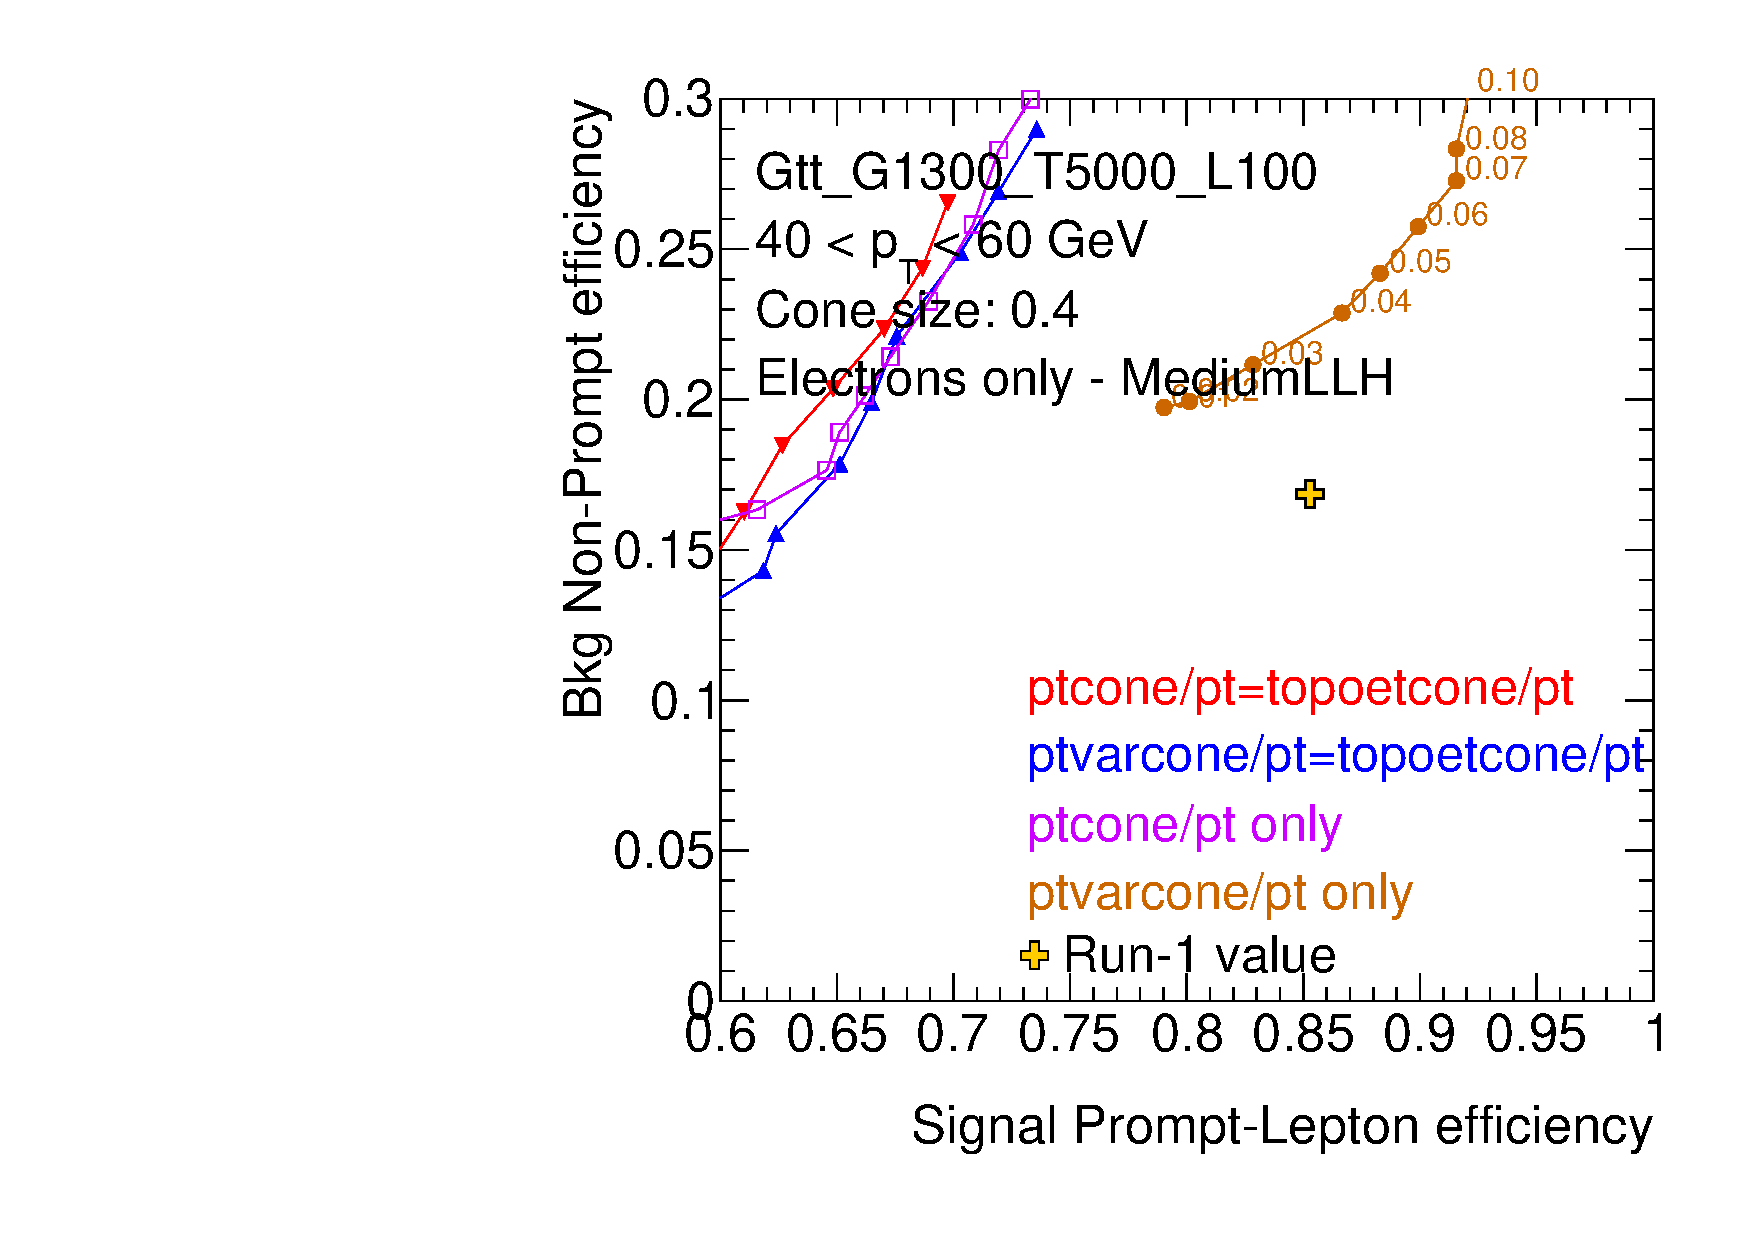
\includegraphics[width=0.4\textwidth]{FIGURES/ISOLATION/Gtt_G1300_T5000_L100_pt3-3_cone40_id11_med.pdf}
\end{center}
\vspace{-0.2cm}
\caption{Isolation efficiency for background non-prompt electrons as a function of the isolation efficiency for prompt electrons in signal events for cone20 (left), cone30 variables (center) and cone30 variables (right). Only electrons with $40<\pt<60$~GeV are shown. Curves are shown for ptcone alone, ptvarcone alone, ptcone combined with topoetcone as well as for ptvarcone combined with topoetcone. In addition, the cross shows the value that would be obtained with settings equivalent to those used during Run-1.}
\label{fig:isoEl1}
\end{figure}

Figure~\ref{fig:isoEl2} and~\ref{fig:isoEl3} compare the performance of the isolation variables including {\tt MediumLLH} and {\tt TightLLH} electron identification. Similar performance is obtained in both cases, although {\tt MediumLLH} 
({\tt TightLLH}) offers a slightly larger signal efficiency at the same rejection at $\pt<60$~GeV ($\pt>60$~GeV). 

\begin{figure}[phtb!]
\begin{center}
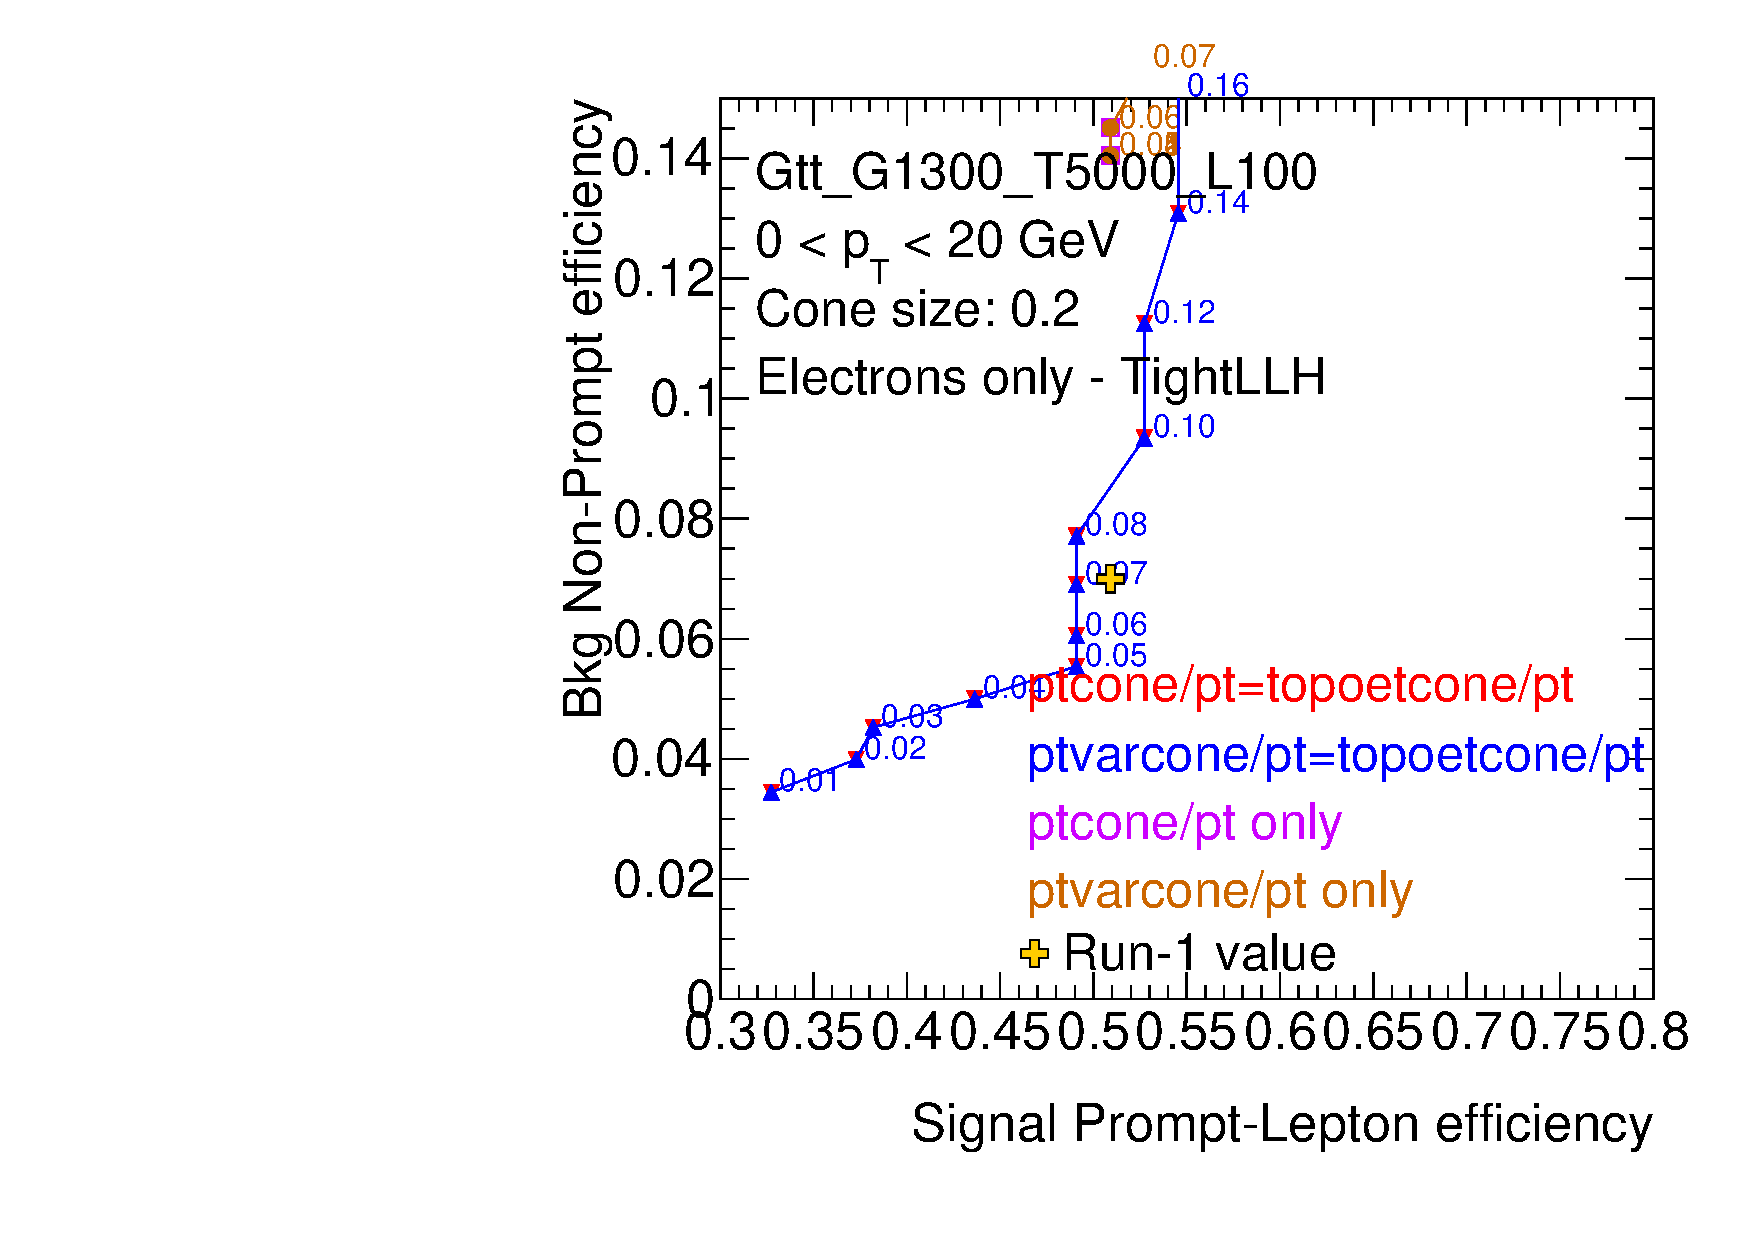
\includegraphics[page=1,width=0.4\textwidth]{FIGURES/ISOLATION/isoEl.pdf}
\includegraphics[page=2,width=0.4\textwidth]{FIGURES/ISOLATION/isoEl.pdf}
\includegraphics[page=3,width=0.4\textwidth]{FIGURES/ISOLATION/isoEl.pdf}
\includegraphics[page=4,width=0.4\textwidth]{FIGURES/ISOLATION/isoEl.pdf}
\includegraphics[page=5,width=0.4\textwidth]{FIGURES/ISOLATION/isoEl.pdf}
\includegraphics[page=6,width=0.4\textwidth]{FIGURES/ISOLATION/isoEl.pdf}
%\includegraphics[page=4,width=0.4\textwidth]{FIGURES/ISOLATION/isoMu.pdf}
%\includegraphics[page=10,width=0.4\textwidth]{FIGURES/ISOLATION/isoMu.pdf}
\end{center}
\vspace{-0.2cm}
\caption{Isolation efficiency for background non-prompt electrons as a function of the isolation efficiency for prompt electrons in signal events for cone20 variables in different electron $\pt$ bins. In addition to the isolation cuts, {\tt TightLLH} (left) and {\tt MediumLLH} (right) identification is also applied. Curves are shown for ptcone alone, ptvarcone alone, ptcone combined with topoetcone as well as for ptvarcone combined with topoetcone. In addition, the cross shows the value that would be obtained with settings equivalent to those used during Run-1.}
\label{fig:isoEl2}
\end{figure}

\begin{figure}[phtb!]
\begin{center}
\includegraphics[page=7,width=0.4\textwidth]{FIGURES/ISOLATION/isoEl.pdf}
\includegraphics[page=8,width=0.4\textwidth]{FIGURES/ISOLATION/isoEl.pdf}
\includegraphics[page=9,width=0.4\textwidth]{FIGURES/ISOLATION/isoEl.pdf}
\includegraphics[page=10,width=0.4\textwidth]{FIGURES/ISOLATION/isoEl.pdf}
\end{center}
\vspace{-0.2cm}
\caption{Isolation efficiency for background non-prompt electrons as a function of the isolation efficiency for prompt electrons in signal events for cone20 variables in different electron $\pt$ bins. In addition to the isolation cuts, {\tt TightLLH} (left) and {\tt MediumLLH} (right) identification is also applied. Curves are shown for ptcone alone, ptvarcone alone, ptcone combined with topoetcone as well as for ptvarcone combined with topoetcone. In addition, the cross shows the value that would be obtained with settings equivalent to those used during Run-1.}
\label{fig:isoEl3}
\end{figure}

\paragraph{Optimization procedure} As concluded form the studies above, the variables to use for the optimization of the isolation are ptvarcone30/$\pt$ in the case of muons, and ptvarcone20/$\pt$ together with topoetcone20/$\pt$ and either {\tt MediumLLH} or 
{\tt TightLLH} for electrons. Appendix~\ref{app_isolation} shows the details of the optimization procedure, which takes into 
account the signal significance for different models for 15 possible isolation definitions. 
This procedure accounts for many details in background and signal samples: combination of lepton $\pt$, 
lepton flavour, prompt and non-prompt combinations of leptons, etc. These studies showed that tight isolation criteria were favoured, 
and therefore the isolation cuts stated in Table~\ref{tab:lepdef} will be used for the analysis: ptvarcone30/\pt\ $<0.06$ for muons; {\tt TightLLH}, ptvarcone20/\pt$<$0.06 and topoetcone20/\pt$<$0.06 for electrons.


\subsubsection{Electron acceptance}
\label{sec:eleAcceptance}

Despite not being included in the object selection employed in this note, dedicated studies have been conducted to evaluate 
the impact of a reduction of the $|\eta|$ coverage for electrons. This is motivated by the fact that the largest contributions 
from charge-flip and fake-lepton backgrounds are observed at $|\eta|>2$ and in the LAr crack region ($1.37<|\eta|<1.52$).

Table~\ref{tab:eleEta} shows the impact on the expected event yields when reducing the electron $|\eta|$ acceptance 
for the two leading electrons (taking a reference the case of $|\eta|<2.3$). The event selection applied to compute those numbers 
requires SS/3L, at least 3 jets with $\pt > 30$~GeV and $m_{ee}$ outside the 84-98~GeV range to reduce the contribution 
from charge flips. 

%%%%%%%%%%%%%%%%%%%%%%%%%%%%%%%%%%%%%%%%%%%%%%%%%%%%%%%%%%%%%
\begin{table}[htb]
\caption{Relative decrease in the event yield when reducing the $|\eta|$ acceptance for the two leading electrons with respect to $|\eta|<2.3$. The reference is considered to be $|\eta|$~$<$~2.47, and the crack region is excluded in all the cases. Numbers are shown for the event selection described in the text and separately for events with 1 or more $b$-jets.}
\label{tab:eleEta}
\begin{center}
    \begin{tabular}{|l|c|c|c|c|c|} \hline
                   & Prompt SS & $\ttbar +W$ & Gtt (G900\_L100) & Non-prompt leptons & Charge flip \\ \hline\hline
==1$b$, $|\eta|<1.37$ & 14\% & 16\% & 12\%  & 28\% & 69\% \\
==1$b$, $|\eta|<2.0$  & 5.4\%  & 6\%  & 7\%&  11\% & 37\% \\ 
==1$b$, $|\eta|<2.3$  & 0.4\%  & 1.5\%  & 4.7\%&  3.6\% &  11\% \\ \hline
$>$1$b$, $|\eta|<1.37$ & 13\% & 18\% & 10\%  & 44\% & 66\% \\
$>$1$b$, $|\eta|<2.0$  & 4.3\%  & 6.5\%  & 2.9\%&  21\% &  30\% \\ 
$>$1$b$, $|\eta|<2.3$  & 1.3\%  & 1.5\%  & 0.3\%&  8\% &  5.8\% \\  \hline
\end{tabular}
\end{center}
\end{table}
%%%%%%%%%%%%%%%%%%%%%%%%%%%%%%%%%%%%%%%%%%%%%%%%%%%%%%%%%%%%

As shown, reducing the acceptance to  $|\eta|<2.0$ would reduce the contribution from processes with prompt 
SS/3L by 6.5\% or less, but the reduction in non-prompt leptons (11-21\%) and and charge flip (30-37\%) is much larger. Also, if reducing 
the acceptance for the two leading electron to $|\eta|<1.37$ would reduce the non-prompt and 
charge flips by 28-44\% and $\sim$69\%, respectively, with a reduction of only 13-18\% in prompt SS/3L processes. 

Therefore, this study proves that additional rejection against some of the main backgrounds affecting the analysis can be achieved 
by reducing the $|\eta|$ acceptance of the electrons, although more work is need to find an optimal selection and minimize 
the impact on signal efficiency.



\subsection{Overlap removal}

According to the above definitions, one single final state object can fall in more than one category, being therefore effectively double-counted. For example, one isolated electron is typically reconstructed both as an electron and as a jet. A procedure to remove overlaps between final state objects was therefore put in place, and applied on pre-selected objects. The recommendations by the Harmonization effort~\cite{Harmonization} have not been applied for this version of the analysis.


First, jets that are angularly close ($\Delta R < 0.2$) to a pre-selected electron are removed from the jet list in the event. Following this, pre-selected electrons (muons) are removed from the electron (muon) list if their distance to the closest jet is $\Delta R < 0.4$. 
%If the distance between two electrons is $\Delta R<0.1$, it is most likely to be that two
%tracks are associated with one calorimeter cluster mistakenly. In this case, lower $E_{\rm T}$ electron 
%is removed. Also 
If there are an electron and muon with $\Delta R<0.1$, it is likely to be the bremsstrahlung
of the muon. Such a muon momentum is not measured correctly so that in this case, both an electron
and a muon are removed.



\subsection{Missing transverse energy}
\label{sec:objects_met}

The missing transverse energy (\met) is rebuilt using the xAOD container ``MET\_RefFinal'' as input and using the calibrated electron, muon and jet objects (and baseline taus and photons according to SUSYTools definitions). In this version of the analysis, the calorimeter soft term is used for building the \met\ following the defaults in SUSYTools-00-05-00-26.


\FloatBarrier

